\documentclass[11pt]{article}


% -- Languages

\newif\ifen
\newif\ifde

% Use \en{Text} for english version text and \de{Text} for german version text
\newcommand{\en}[1]{\ifen#1\fi}
\newcommand{\de}[1]{\ifde#1\fi}

% Uncomment for english version
\entrue

% Uncomment for german version
%\detrue

% -- Color scheme

% Color package
\usepackage{xcolor}

% Color definitions
\definecolor{minimal-gray}{HTML}{f2f2f2}
\definecolor{minimal-black}{HTML}{131313}
\definecolor{minimal-white}{HTML}{F3F2F5}
\definecolor{minimal-red}{HTML}{C43C2D}
\definecolor{minimal-blue}{HTML}{343454}
\definecolor{minimal-yellow}{HTML}{F1C40F}
\definecolor{minimal-green}{HTML}{2D6514}
\definecolor{minimal-beige}{HTML}{D7B6A5}

% Colorbox environments
\usepackage[most]{tcolorbox}


% -- Page layout

% Layout adjustments of page (a4 without margin)
\usepackage[paperheight=842pt, paperwidth=595pt, margin=0pt]{geometry}

% Remove paragraph indentation
\setlength{\parindent}{0pt}

% Interline spacing options
\newcommand{\largespace}{\\[2pt]}
\newcommand{\mediumspace}{\\[-3pt]}
\newcommand{\smallspace}{\\[-5pt]}

% In-box spacing around content
\newcommand{\inboxspacing}{.015\paperheight}

% Horizontal spacing of the boxes (must sum up to 1)
\newcommand{\sideboxwidth}{.35}
\newcommand{\mainboxwidth}{.65}

% Vertical spacing of the boxes (must sum up to 1)
\newcommand{\headboxheight}{.070}
\newcommand{\mainboxheight}{.910}
\newcommand{\footboxheight}{.020}

%   sideboxwidth           mainboxwidth
%  <------------> <---------------------------->
%  _____________________________________________
% |#############################################| ^
% |#######  #  # #  ## # #  #  #     # #########| |
% |####### # # # # # # # # # # # ### # #########| | headboxheight
% |####### ### # # ##  # # ### # # # #   #######| |
% |#############################################| v
% |///////////////                              | ^
% |///////////////                              | |
% |///////////////                              | |
% |///////////////                              | |
% |///////////////                              | |
% |///////////////                              | |
% |///////////////                              | |
% |///////////////                              | |
% |///////////////                              | | mainboxheight
% |///////////////                              | |
% |///////////////                              | |
% |///////////////                              | |
% |///////////////                              | |
% |///////////////                              | |
% |///////////////                              | |
% |///////////////                              | |
% |///////////////                              | v
% |#############################################| ^
% |#############################################| | footboxheight
% |#############################################| v


% -- Font settings

% Typesetting packages
\usepackage[letterspace=20]{microtype}
\usepackage[T1]{fontenc}

% Raleway font family
\usepackage[semibold]{raleway}
\renewcommand{\familydefault}{\sfdefault}

% Custom font commands
\newcommand{\header}[2]{\uppercase{\textbf{\fontsize{30}{100}{\lsstyle{#1 \hspace{3pt} #2}}}}}
\newcommand{\titlefont}[1]{\uppercase{\textbf{\Large{#1}}}}


% -- Additional packages

% Multirow tables
\usepackage{multirow}

% Settings for entire table columns (e.g \begin{tabular}{>{\footnotesize}rl})
\usepackage{array}

% Tikzpicture graphics
\usepackage{tikz}

% Clickable URLs
\usepackage{hyperref}
\urlstyle{same}


\begin{document}

\begin{tcbposter}[
    poster = {columns=1, rows=1, spacing=0pt},
    boxes = {sharp corners, halign=center, valign=center, boxrule=0pt}
]


% -- Headbox

\posterbox[
    colback=minimal-black,
    halign=center]
    {name=headbox,
    span=1,
    rowspan=\headboxheight}
{

    \color{white}

    \header{Fabio}{Matti}

    \vspace{-8px}
    \hspace{2px}
    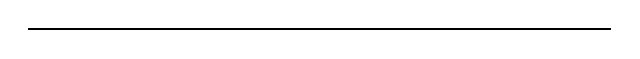
\begin{tikzpicture}
        \draw[fill=white] (-3.7, -0.01) rectangle (3.7, 0.01);
    \end{tikzpicture}
    \vspace{1px}

    \en{\titlefont{Computational Scientist}}
    \de{\titlefont{Stellenbezeichnung oder Firmenname}}
}


% -- Sidebox

\posterbox[
    colback=minimal-gray,
    valign=top,
    top=\inboxspacing,
    halign=right,
    right=\inboxspacing]
    {name=sidebar,
    below=headbox,
    column=1,
    span=\sideboxwidth,
    rowspan=\mainboxheight}
{

    \begin{tabular}{rl}

        \multicolumn{2}{@{}c@{}}{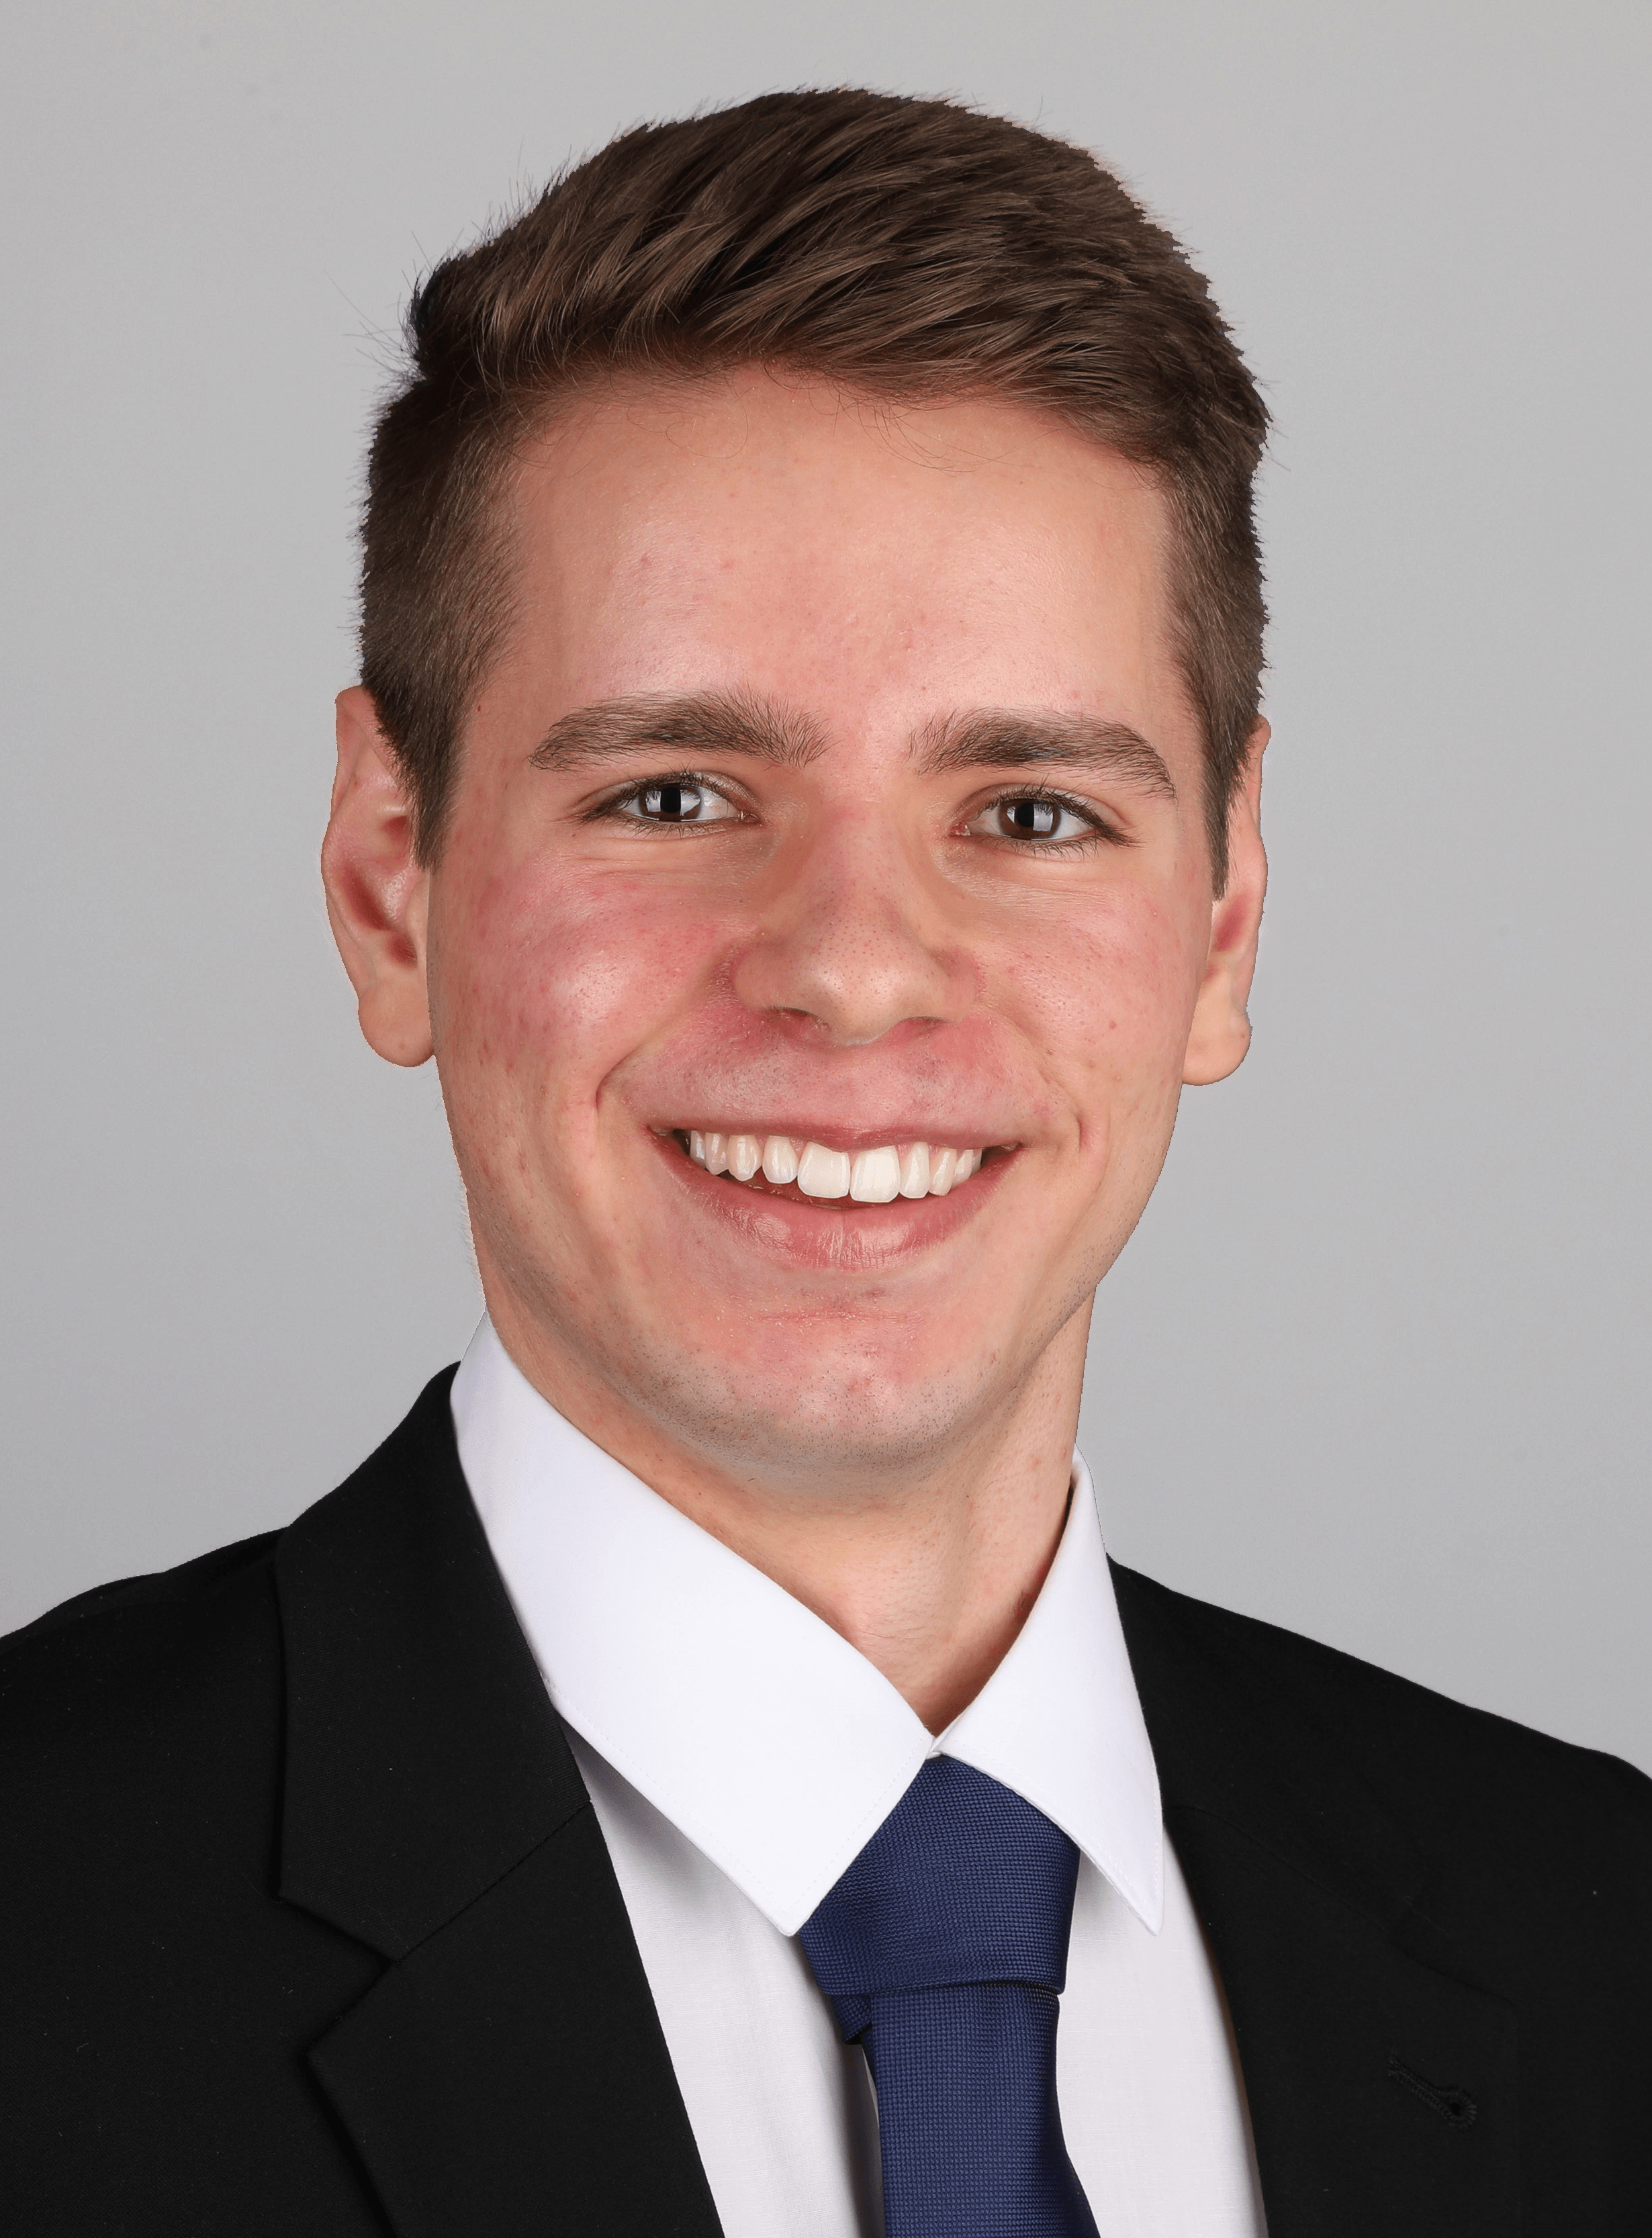
\includegraphics[scale=0.07]{images/formal_final.png}} \\ \mediumspace

        & \titlefont{\en{Contact}\de{Kontakt}} \\ \hline \mediumspace

        \multirow{4}{*}{\scalebox{0.075}{
\begin{tikzpicture}

    % Background
    \fill[minimal-black] (0, 0) circle (7);
  
    % Foundation
    \fill[minimal-white] (-3.2, -5.3) rectangle (3.2, -4.7);

    % Houses
    \fill[minimal-white] (-2.8, -4.3) rectangle (-0.8, -1.4);
    \fill[minimal-white] (0.4, -4.3) rectangle (2.8, -2.6);
    \fill[minimal-white] (-0.4, -4.3) -- (0.0, -4.3) -- (0.0, -2.2) -- (0.6, -2.2) -- (0.6, 1.0) -- (-1.6, 1.0) -- (-1.6, -1.0) -- (-0.4, -1.0) -- cycle;

    % Tower
    \fill[minimal-white] (1.0, -2.2) -- (2.0, -2.2) -- (2.0, 2.6) -- (-0.4, 2.6) -- (-0.4, 1.4) -- (1.0, 1.4) -- cycle;
    \fill[minimal-white] (0.2, 3.0) rectangle (1.4, 3.8);
    \fill[minimal-white] (0.6, 4.2) rectangle (1.0, 5.3);
    
\end{tikzpicture}}}
            & \textbf{\en{Address}\de{Adresse}} \\
                %& Bürgstrasse 56 \\
                %& 3700 Spiez \\
                & Route Cantonale 99A \\
                & 1025 Saint-Sulpice \\
                & \smallspace

        \multirow{2}{*}{\scalebox{0.075}{
\begin{tikzpicture}
    
    % Background
    \fill[minimal-black] (0, 0) circle (7);

    % Shell
    \fill[minimal-white] (-3.2, -5.3) rectangle (3.2, 5.3);
    \fill[minimal-black] (-2.8, -4.7) rectangle (2.8, 4.9);
    \fill[minimal-white] (-2.4, -4.3) rectangle (2.4, 4.5);

    % Button
    \fill[minimal-black] (-0.9, -5.1) rectangle (0.9, -3.9);
    \fill[minimal-white] (-0.5, -4.7) rectangle (0.5, -4.3);

\end{tikzpicture}}}
            & \textbf{\en{Phone}\de{Telefon}} \\
                & \href{tel:+41793211310}{+41 79 321 13 10} \\
                & \smallspace

        \multirow{2}{*}{\scalebox{0.075}{
\begin{tikzpicture}

    % Background
    \fill[minimal-black] (0, 0) circle (7);
  
    % Foundation
    \fill[minimal-white] (-3.2, -5.3) rectangle (3.2, -4.7);

    % Letter
    \fill[minimal-white] (-2.8, -4.3) -- (2.8, -4.3) -- (2.8, -0.8) -- (0.0, -3.6) -- (-2.8, -0.8) -- cycle;
    \fill[minimal-white] (-2.8, -0.4) -- (0.0, -3.2) -- (2.8, -0.4) -- cycle;

    % Arrow
    \fill[minimal-white] (-0.8, 5.3) -- (-0.8, 2.4) -- (-1.8, 2.4) -- (0.0, 0.6) -- (1.8, 2.4) -- (0.8, 2.4) -- (0.8, 5.3) -- cycle;

\end{tikzpicture}}}
            & \textbf{E-Mail} \\
                & \href{mailto:fabio.matti@bluewin.ch}{fabio.matti@bluewin.ch} \\
                & \largespace

        & \titlefont{\en{Personal}\de{Persönliches}} \\ \hline \mediumspace

        \multirow{2}{*}{\scalebox{0.075}{
\begin{tikzpicture}
    
    % Background
    \fill[minimal-black] (0, 0) circle (7);
  
    % Foundation
    \fill[minimal-white] (-3.2, -5.3) rectangle (3.2, -4.7);

    % Base
    \fill[minimal-white] (-2.8, -4.3) -- (-2.8, -1.4) -- (0.4, -1.4) -- (0.4, -3.6) -- (1.6, -3.6) -- (1.6, -2.6) -- (2.4, -2.6) -- (2.4, -1.4) -- (2.8, -1.4) -- (2.8, -4.3) -- cycle;
    
    % Cream
    \fill[minimal-white] (-3.2, -1.0) -- (-3.2, 0.0) -- (3.2, 0.0) -- (3.2, -1.0) -- (2.0, -1.0) -- (2.0, -2.2) -- (1.2, -2.2) -- (1.2, -3.2) -- (0.8, -3.2) -- (0.8, -1.0) -- cycle;
      
    % Candles
    \fill[minimal-white] (-2.6, 0.4) rectangle (-2.0, 3.4);
    \fill[minimal-white] (-2.5, 3.8) rectangle (-2.1, 4.6);

    \fill[minimal-white] (-0.6, 0.4) rectangle (0.0, 2.2);
    \fill[minimal-white] (-0.5, 2.6) rectangle (-0.1, 3.4);

    \fill[minimal-white] (-1.4, 0.4) --  (-1.0, 0.4) -- (-1.0, 2.6) --  (-0.8, 2.6) --  (-0.8, 4.0) -- (-1.4, 4.0) -- cycle;
    \fill[minimal-white] (-1.3, 4.4) rectangle (-0.9, 5.2);
    
    \fill[minimal-white] (0.8, 0.4) rectangle (1.4, 3.6);
    \fill[minimal-white] (0.9, 4.0) rectangle (1.3, 4.8);
    
    \fill[minimal-white] (2.0, 0.4) rectangle (2.6, 2.8);
    \fill[minimal-white] (2.1, 3.2) rectangle (2.5, 4.0);

\end{tikzpicture}}}
            & \textbf{\en{Date of Birth}\de{Geburtsdatum}} \\
                & 30/08/1998 \\
                & \smallspace

        \multirow{2}{*}{\scalebox{0.075}{
\begin{tikzpicture}

    % Background
    \fill[minimal-black] (0, 0) circle (7);

    % Foundation
    \fill[minimal-white] (-3.2, -5.3) rectangle (3.2, -4.7);

    % Pole
    \fill[minimal-white] (-2.4, -4.3) rectangle (-2.0, 4.5);
    \fill[minimal-white] (-2.6, 4.9) rectangle (-1.8, 5.3);
    
    % Fabric
    \fill[minimal-white] (-0.2, 0.8) -- (3.0, 0.8) -- (3.0, 3.9) -- (1.4, 3.9) -- (1.4, 1.2) -- (-0.2, 1.2) -- cycle; 
    \fill[minimal-white] (-1.6, 1.6) rectangle (1.0, 4.5);
    
\end{tikzpicture}}}
            & \textbf{\en{Nationality}\de{Nationalität}} \\
                & \en{Swiss}\de{Schweiz} \\
                & \largespace

        & \titlefont{\en{Platforms}\de{Platformen}} \\ \hline \mediumspace

        \multirow{2}{*}{\scalebox{0.075}{
\begin{tikzpicture}

    % Background
    \fill[minimal-black] (0, 0) circle (7);

    % Foundation
    \fill[minimal-white] (-3.2, -5.3) rectangle (3.2, -4.7);

    % Logo
    \fill[minimal-white] (1.7, -4.3) -- (-1.7, -4.3) to[out=90, in=270] (-1.675, -4.05)
                                             to[out=190, in=330] (-3.6, -3.8)
                                             to[out=150, in=330] (-4.6, -2.35) % Tail
                                             to[out=150, in=280] (-5.0, -1.9) % Tail
                                             to[out=20, in=140] (-4.0, -2.1) % Tail
                                             to[out=320, in=160] (-3.0, -3.2) % Tail
                                             to[out=340, in=210] (-1.7, -3.1) % Tail
                                             to[out=80, in=230] (-1.25, -2.2) % Shoulder (left)
                                             to[out=180, in=230, looseness=1.15] (-3.6, 3.1) % Cheek (left)
                                             to[out=110, in=250] (-3.5, 4.9) % Ear (left)
                                             to[out=340, in=130] (-1.8, 4.1) % Ear (left)
                                             to[out=15, in=165] (1.8, 4.1) % Top
                                             to[out=50, in=200] (3.5, 4.9) % Ear (right)
                                             to[out=290, in=70] (3.6, 3.1) % Ear (right)
                                             to[out=310, in=0, looseness=1.15] (1.25, -2.2) % Cheek (right)
                                             to[out=310, in=100] (1.7, -3.1) % Shoulder (right)
                                             -- cycle;

\end{tikzpicture}}}
            & \textbf{GitHub} \\
                & \href{https://github.com/FMatti}{github.com/FMatti} \\
                & \smallspace

        \multirow{2}{*}{\scalebox{0.075}{
\begin{tikzpicture}
    
    % Background
    \fill[minimal-black] (0, 0) circle (7);

    % i-base
    \fill[minimal-white] (-4.0, -4.0) rectangle (-2.3, 1.2);

    % i-dot
    \fill[minimal-white] (-3.15, 3.2) circle (1.0);

    % n
    \fill[minimal-white] (-1.2, -4.0) -- (-1.2, 1.2) -- (0.5, 1.2) -- (0.5, 0.5)
                 to[out=50, in=100, looseness=1.3] (4.0, -0.5)
                 -- (4.0, -4.0) -- (2.3, -4.0) -- (2.3, -0.7) 
                 to[out=100, in=80, looseness=1.1] (0.5, -0.8) -- (0.5, -4.0) -- cycle;

\end{tikzpicture}}}
            & \textbf{LinkedIn} \\
                & \href{https://linkedin.com/in/fmatti}{linkedin.com/in/FMatti} \\
                & \largespace

        & \titlefont{\en{Languages}\de{Sprachen}} \\ \hline \mediumspace

        \multirow{2}{*}{\scalebox{0.075}{
\begin{tikzpicture}

    % Clip mask
    \clip (0, 0) circle (7);

    % Red
    \fill[minimal-red] (-7, -2.4) rectangle (7, 2.4);
    
    % Black
    \fill[minimal-black] (-7, 2.4) rectangle (7, 7);
    
    % Yellow
    \fill[minimal-yellow] (-7, -7) rectangle (7, -2.4);
    
\end{tikzpicture}
}}
            & \textbf{\en{German}\de{Deutsch}} \\
                & \en{Native}\de{Muttersprache} \\
                & \smallspace

        \multirow{2}{*}{\scalebox{0.075}{
\begin{tikzpicture}

    % Clip mask
    \clip (0, 0) circle (7);

    % Background
    \fill[minimal-blue] (0, 0) circle (7);

    % Diagonal
    \fill[minimal-white, rotate around={38.5:(0, 0)}] (-7.5, -1.1) rectangle (7.5, 1.1);
    \fill[minimal-red, rotate around={38.5:(0, 0)}] (0.0, 0.2) rectangle (7.5, 0.9);
    \fill[minimal-red, rotate around={38.5:(0, 0)}] (-7.5, -0.9) rectangle (0.0, -0.2);
    
    \fill[minimal-white, rotate around={-38.5:(0, 0)}] (-7.5, -1.1) rectangle (7.5, 1.1);
    \fill[minimal-red, rotate around={-38.5:(0, 0)}] (0.0, 0.2) rectangle (7.5, 0.9);
    \fill[minimal-red, rotate around={-38.5:(0, 0)}] (-7.5, -0.9) rectangle (0.0, -0.2);
    
    % Cross
    \fill[minimal-white] (-7.5, -1.8) rectangle (7.5, 1.8);
    \fill[minimal-white] (-1.8, -7.5) rectangle (1.8, 7.5);

    \fill[minimal-red] (-7.5, -1.25) rectangle (7.5, 1.25);
    \fill[minimal-red] (-1.25, -7.5) rectangle (1.25, 7.5);

\end{tikzpicture}
}}
            & \textbf{\en{English}\de{Englisch}} \\
                & \en{Proficient}\de{Ausgezeichnet} (CEFR: C2) \\
                & \smallspace

        \multirow{2}{*}{\scalebox{0.075}{
\begin{tikzpicture}

    % Clip mask
    \clip (0, 0) circle (7);

    % White
    \fill[minimal-white] (-2.4, -7) rectangle (2.4, 7);
    
    % Red
    \fill[minimal-red] (2.4, -7) rectangle (7, 7);
    
    % Blue
    \fill[minimal-blue] (-7, -7) rectangle (-2.4, 7);
    
\end{tikzpicture}}}
            & \textbf{\en{French}\de{Französisch}} \\
                & \en{Fluent}\de{Sehr gut} (CEFR: C1)

    \end{tabular}
}


% -- Mainbox

\posterbox[
    colback=white,
    valign=top,
    top=\inboxspacing,
    halign=left,
    left=\inboxspacing]
    {name=mainbox,
    column*=1,
    span=\mainboxwidth,
    below=headbox,
    rowspan=\mainboxheight}
{

    \color{minimal-black}

    \begin{tabular}{>{\footnotesize}rl}

        & \titlefont{\en{Education}\de{Bildungsweg}} \\ \hline \mediumspace

        \en{Since}\de{Seit} 09/2021
            & \en{\textbf{EPFL, Master's studies}}
            \de{\textbf{EPFL, Masterstudium}} \\
            & Computational Science (74 ECTS, GPA: 5.60) \\
            & \smallspace

        09/2018 - 07/2021
            & \en{\textbf{University of Bern, Bachelor of Science}}
            \de{\textbf{Universität Bern, Bachelor of Science}}\\
            & \en{Physics (Major, 120 ECTS, GPA: 5.80)}
            \de{Physik (Major, 120 ECTS, Note: 5.80)}\\
            & \en{Mathematics (Minor, 71 ECTS, GPA: 5.68)}
            \de{Mathematik (Minor, 71 ECTS, Note: 5.68)} \\
            & \largespace

        & \titlefont{\en{Expericence}\de{Erfahrung}} \\ \hline \mediumspace

        07/2022 - 09/2022
            & \textbf{Omnisens S.A. (Prysmian Group), Morges} \\
            & \textbf{Machine learning internship} \\
            & Designed of efficient data reduction methods \\
            & Implemented anomaly detection algorithms \\
            & \largespace

        & \titlefont{\en{Projects}\de{Projekte}} \\ \hline \mediumspace

        Semester Project
            & \textbf{Rational Interpolation of Maxwell's equations} \\
            & Finite element method, model order reduction \\
            & \href{https://github.com/FMatti/Maxwell-MRI}{github.com/FMatti/Maxwell-MRI} \\
            & \smallspace
        Bachelor's Thesis
            & \textbf{Learned Spectral Decoloring in Photoacoustics} \\
            & Gradient boosting, feature importance \\
            & \href{https://github.com/FMatti/ALE-LSD}{github.com/FMatti/ALE-LSD} \\
            & \largespace

        & \titlefont{\en{Activities}\de{Tätigkeiten}} \\ \hline \mediumspace

        \en{Since}\de{Seit} 09/2022
            & \en{\textbf{Machine Learning Student Assistant}}
            \de{\textbf{Assistent für Machine Learning}} \\
            & \en{Master course on fundamental ML methods} \\
            & \smallspace
        
        \en{Since}\de{Seit} 09/2022
            & \en{\textbf{Programming Concepts Student Assistant}}
            \de{\textbf{Assistent für Programming Concepts}} \\
            & \en{Master course in C\texttt{++} and scientific computing} \\
            & \smallspace
        
        \en{Since}\de{Seit} 06/2018
            & \en{\textbf{NBC Staff Officer in the Air Base Command 13}}
            \de{\textbf{ABC Stabsoffizier im Flugplatzkommando 13}} \\
            & \en{Leadership assistant of battalion commander} \\
            & \en{In charge of NBC instruction of 700 soldiers}
            \de{Zuständig für ABC Ausbildung von 700 Soldaten} \\
            & \smallspace

        \en{Since}\de{Seit} 12/2014
            & \en{\textbf{Alpine Skiing Teacher for Skiclub Zweisimmen}}
            \de{\textbf{Skilehrer für den Skiklub Zweisimmen}} \\
            & \largespace

        & \titlefont{\en{Qualifications}\de{Zertifikate}} \\ \hline \mediumspace

        02/2020     & \en{\textbf{Cambridge C2 Proficiency English (Grade: A)}}
                    \de{\textbf{Cambridge C2 Proficiency English (Note: A)}} \\
        07/2019     & \en{\textbf{GRE General Test (V: 157, Q: 167, AW: 5.5)}}
                    \de{\textbf{GRE General Test (V: 157, Q: 167, AW: 5.5)}} \\
        09/2018     & \en{\textbf{SVF Leadership Certificate}}
                    \de{\textbf{SVF Leadership Zertifikat}} \\
                    & \largespace

        & \titlefont{\en{Computational Skills}\de{IT-Kenntnisse}} \\ \hline \mediumspace

            \en{Programming}\de{Programmierung}
                & \textbf{\en{Proficient}\de{Experte}}: Python, C\texttt{++}, \LaTeX \\
                & \textbf{\en{Advanced}\de{Fortgeschritten}}: C, R, MATLAB \\

            Software
                & \textbf{\en{Proficient}\de{Experte}}: Git, Microsoft Office, GIMP \\
                & \textbf{\en{Advanced}\de{Fortgeschritten}}: Blender, Inkscape, Photoshop \\
                & \largespace

        & \titlefont{Hobbies} \\ \hline \mediumspace
            & \en{Skiing, Running, Graphic Design, Reading}
            \de{Skifahren, Running, Graphic Design, Lesen} \\

    \end{tabular}
}


% -- Footbox

\posterbox[colback=minimal-black]
           {name=blankbox2,
           below=sidebar,
           column=1,
           span=1,
           rowspan=\footboxheight}{
           
    \color{white}
    {\tiny Find the source code and a digital version of this CV at \href{https://github.com/FMatti/Personal-CV}{github.com/FMatti/Personal-CV} }

}

\end{tcbposter}

\end{document}
